\section{Dispersion relations for concrete graph topologies} \label{sec:Examples}
Throughout this section, we are concerned with determining the spectrum of the problem \eqref{eq:WholeSpaceLaplaceEqn}, via the spectra of \eqref{eq:QGFullSystem}, for $\qm\in\left[-\pi,\pi\right)$.
The examples we consider in this section are chosen to highlight how the properties of the spectrum vary on both the placement of coupling constants at the vertices, as well as the geometry of the singular-structures themselves. 

\subsection{One-Dimensional Loop} \label{ssec:Example1DLoop}
We begin with the simplest example: a ``chain" of vertices that is periodic in one direction.
Its purpose is mainly to be used to draw contrast with the following example in section \ref{ssec:EmbeddingDependentExample}, where we will show that adding additional ``pieces" to the chain can cause spectral gaps to open.
However this example is also useful as a conceptual demonstration of how one takes the period graph of a physical singular-structure and employs proposition \ref{prop:M-MatrixEntries} to construct the $M$-matrix and extract the spectral information.

Consider the graph $\graph$ periodic in one direction (without loss of generality assumed parallel to the $x_1$-axis with $x_2=0$) in $\reals\times\sqbracs{0,1}$, with vertices $v_j = \bracs{j + \recip{2}, 0}^\top$ and edges $I_{j\bracs{j+1}}$ for $j\in\integers$.
Note that since $\graph$ is only periodic in the $x_1$-direction, the period cell lies in $S^1\times\sqbracs{0,1}$ rather than the usual 2D-torus for a graph periodic in two directions in $\reals^2$.
We also only have a scalar quasi-momentum $\qm\in\left[-\pi,\pi\right)$ (one can set $\qm_2=0$ in \eqref{eq:QGFullSystem} when constructing the $\qm_{jk}$ to account for the lack of periodicity in $x_2$).
Assume the coupling constants at each vertex are identical, taking the value $\alpha\in\reals$.
Then the quantum graph which corresponds to the period graph of $\graph$ is simply a single vertex $v$ with a looping edge $I$ of length 1, with quasi-momentum $\qm$ on $I$ and coupling constant $\alpha$ at $v$. 
One can apply proposition \ref{prop:M-MatrixEntries} at this point to compute the (one-dimensional) $M$-matrix, however for illustrative purposes (and consistency with the examples that follow), we elect to introduce an artificial vertex to break the loop $I$ into two edges, producing a new quantum graph $\graph_{\mathcal{P}}=\bracs{\vertSet, \edgeSet}$ with
\begin{align*}
	\vertSet = \clbracs{ v_1 , v_2 }, \quad \edgeSet = \clbracs{ I_{12}, I_{21} },
	&\qquad \abs{I_{12}} = \abs{I_{21}} = \recip{2}, \quad \qm_{12} = \qm_{21} = \qm, 
	&\qquad \alpha_1 = \alpha, \quad &\alpha_2 = 0.
\end{align*}
We illustrate the process of moving from $\graph$ to $\graph_{\mathcal{P}}$ in figure \ref{fig:Diagram_1DExample}.
Note that the artificial vertex having coupling constant equal to zero ensures that the incoming edge solutions and their derivatives match at $v_2$, ensuring that introducing $v_2$ does not alter the behaviour of solutions along the ``cut loop".
Studying the $M$-matrix of $\graph_{\mathcal{P}}$ to determine the eigenvalues $\omega^2$ is now equivalent to studying the spectrum of the original problem.
\begin{figure}[b]
	\centering
	\begin{subfigure}[t]{0.3\textwidth}
		\centering
		\includegraphics[scale=2]{Diagram_1DLineGraph.pdf}
		\caption{\label{fig:Diagram_1DLineGraph} The graph $\graph$, periodic in one dimension, consisting of integer-spaced vertices.}
	\end{subfigure}
	~
	\begin{subfigure}[t]{0.3\textwidth}
		\centering
		\includegraphics[scale=2]{Diagram_1DLineQuantumGraph.pdf}
		\caption{\label{fig:Diagram_1DLineQuantumGraph} The corresponding quantum graph of the period cell of $\graph$, containing one (looping) edge of length 1}
	\end{subfigure}
	~
	\begin{subfigure}[t]{0.3\textwidth}
		\centering
		\includegraphics[scale=2]{Diagram_1DLineComputationGraph.pdf}	
		\caption{\label{fig:Diagram_1DLineComputationGraph} The equivalent graph $\graph_{\mathcal{P}}$ that we study. Note that the dummy vertex $v_2$ has coupling constant 0.}
	\end{subfigure}
	\caption{\label{fig:Diagram_1DExample} The graphs $\graph$ and $\graph_{\mathcal{P}}$.}
\end{figure} \newline

One can construct the $M$-matrix for $\graph_{\mathcal{P}}$ using proposition \ref{prop:M-MatrixEntries}, obtaining
\begin{align*}
	M_{\qm}\bracs{\omega^2} &= 
	\begin{pmatrix}[1.75]
		2\omega\cot\dfrac{\omega}{2} & -2\omega\csc\dfrac{\omega}{2}\cos\dfrac{\qm}{2} \\
		-2\omega\csc\dfrac{\omega}{2}\cos\frac{\qm}{2} & 2\omega\cot\dfrac{\omega}{2}
	\end{pmatrix}.
\end{align*}
The matrix of coupling constants is $A = \mathrm{diag}\bracs{\alpha, 0}$, so we work with the matrix
\begin{align*}
	\tilde{M}_\qm\bracs{\omega^2} &= 
	\begin{pmatrix}[1.75]
		2\omega\cot\dfrac{\omega}{2} - \alpha\omega^2 & -2\omega\csc\dfrac{\omega}{2}\cos\dfrac{\qm}{2} \\
		-2\omega\csc\dfrac{\omega}{2}\cos\dfrac{\qm}{2} & 2\omega\cot\dfrac{\omega}{2}		
	\end{pmatrix},
\end{align*}
and solve either $\tilde{M}_\qm\bracs{\omega^2} w = 0$ for eigenpairs $\bracs{\omega^2, w}$, or $\det\tilde{M}_\qm \bracs{\omega^2} = 0$ for the eigenvalues $\omega^2$.
With $\tilde{M}_\qm$ being a relatively small matrix, taking the latter approach is feasible analytically, and one can obtain the following equation for $\omega$ for a given $\qm$:
\begin{align*}
	\cos\qm &= \cos\omega - \frac{\alpha\omega}{2}\sin\omega.
\end{align*}
We would then need to determine, for each $\qm\in\left[-\pi, \pi\right)$, the set of solutions for $\omega$ and then take the union to provide the spectrum of our original problem.
This procedure is similar to that in example \ref{ssec:ExampleCrossInPlane}, which we will study in greater depth, and as one might expect produces a qualitatively similar spectrum.

\subsection{``Decorated" Graph with Dependencies Arising from the Embedding} \label{ssec:EmbeddingDependentExample}
We next provide an explicit example to complement the discussion that concluded section \ref{ssec:MMatrix} as well as demonstrate that adding additional edges to a graph can be used to open gaps in the resulting spectrum.
Because of the need to distinguish between two objects that bear similar names, we will prefix the term ``quantum graph" with ``(embedded)" when we are discussing an quantum graph that has been equipped with an embedding, and will use the prefix ``(abstract)" when we wish to refer to a quantum graph that has yet to be assigned an embedding.

Consider the (embedded) graph $\graph$ periodic in one direction (without loss of generality assumed parallel to the $x_1$-axis with $x_2=0$) in $\reals\times\sqbracs{0,1}$, with vertices
\begin{align*}
	v_1^m = \bracs{m + \recip{2}, \recip{2}}^\top, 
	&\quad v_2^m = \bracs{m + \recip{2}\bracs{1+\cos\beta}, \recip{2}\bracs{1+\sin\beta}}^\top,
\end{align*}
for a fixed angle $\beta\in\bracs{0,\pi}$, and edges $I_{1}^{m} = \sqbracs{v_1^m, v_1^{m+1}}$ and $I_{12}^m=\sqbracs{v_1^m, v_2^m}$ for $m\in\integers$.
Place a single coupling constant with value $\alpha$ at each $v_1^m$, and assume that $v_2^m$ has coupling constant zero for each $m$.
Then the (abstract) quantum graph which corresponds to the (embedded) period graph of $\graph$ consists of two vertices and two edges, with one of the edges being a loop.
However it is important to note that the (abstract) quantum graph does not contain any reference to the angle $\beta$ at which the edge connecting the two vertices is orientated at --- this is entirely an artefact of our decision to embed this graph into $\reals\times\sqbracs{0,1}$.
We again elect to introduce an artificial vertex to obtain an equivalent (embedded) quantum graph $\graph_{\mathcal{P}}$ which describes the (embedded) period graph of $\graph$:
\begin{align*}
	&\graph_{\mathcal{P}} = \bracs{\vertSet, \edgeSet}, \quad
	\vertSet = \clbracs{ v_1, v_2, v_3 }, \quad
	\edgeSet = \clbracs{ I_{12}, I_{13}, I_{31} }, \\
	&v_1 = \bracs{\recip{2},\recip{2}}, \quad
	v_2 = \bracs{\recip{2}\bracs{1+\cos\beta}, \recip{2}\bracs{1+\sin\beta}}, \quad
	v_3 = \bracs{1, \recip{2}}.
\end{align*}
The process of moving from $\graph$ to $\graph_{\mathcal{P}}$ is illustrated in figure \ref{fig:Diagram_1DAngledEdgeExample}.
\begin{figure}[b]
	\centering
	\begin{subfigure}[t]{0.3\textwidth}
		\centering
		\includegraphics[scale=1.85]{Diagram_1DAngledEdge-Embedded.pdf}
		\caption{\label{fig:Diagram_1DAngledEdge-Embedded} The graph $\graph$, periodic in one dimension, consisting of integer-spaced vertices with an edge ``hanging" at an angle $\beta$.}
	\end{subfigure}
	~
	\begin{subfigure}[t]{0.3\textwidth}
		\centering
		\includegraphics[scale=1.85]{Diagram_1DAngledEdge-Quantum.pdf}
		\caption{\label{fig:Diagram_1DAngledEdge-Quantum} The corresponding quantum graph of the period cell of $\graph$, containing one (looping) edge of length 1 and another edge connecting the two vertices.}
	\end{subfigure}
	~
	\begin{subfigure}[t]{0.3\textwidth}
		\centering
		\includegraphics[scale=1.85]{Diagram_1DAngledEdge-Computation.pdf}	
		\caption{\label{fig:Diagram_1DAngledEdge-Computation} The equivalent graph $\graph_{\mathcal{P}}$ that we study. Note that the dummy vertex $v_3$ has coupling constant 0.}
	\end{subfigure}
	\caption{\label{fig:Diagram_1DAngledEdgeExample} The graphs $\graph$ and $\graph_{\mathcal{P}}$.}
\end{figure}

Since $\graph_{\mathcal{P}}$ is periodic in the $x_1$-direction with period 1, we have a scalar quasi-momentum $\qm\in\left[-\pi,\pi\right)$ with
\begin{align*}
	\qm_{13} = \qm_{31} = \qm, \quad \qm_{12} = \qm\cos\beta,
\end{align*}
and still have a coupling constant $\alpha$ at $v_1$. 
One can apply proposition \ref{prop:M-MatrixEntries} at this point to compute the $M$-matrix corresponding to the problem \eqref{eq:QGFullSystem} on $\graph_{\mathcal{P}}$, obtaining
\begin{align} \label{eq:EmbeddedGraphMMatrix}
	M_\qm\bracs{\omega^2} &=
	\begin{pmatrix}[1.75]
		3\omega\cot\dfrac{\omega}{2} & -\omega \exp\bracs{\dfrac{\rmi\qm\cos\beta}{2}}\csc\dfrac{\omega}{2} & -2\omega\csc\dfrac{\omega}{2}\cos\dfrac{\qm}{2} \\
		-\omega \exp\bracs{-\dfrac{\rmi\qm\cos\beta}{2}}\csc\dfrac{\omega}{2} & \omega\cot\dfrac{\omega}{2} & 0 \\
		-2\omega\csc\dfrac{\omega}{2}\cos\frac{\qm}{2} & 0 & 2\omega\cot\dfrac{\omega}{2}
	\end{pmatrix}.
\end{align}
Here it can be seen that the angle $\beta$ has entered into the form of the $M$-matrix due to our choice of embedding, in particular the manner in which we chose to embed the vertex $v_2$ and edge $I_{12}$.
However we will see that the spectrum of \eqref{eq:QGFullSystem} on $\graph$ is independent of $\beta$, as one would expect from examining its (abstract) periodic quantum graph in the alternative manner described in section \ref{ssec:MMatrix}.

The matrix of coupling constants is $A=\mathrm{diag}\bracs{\alpha, 0, 0}$, so one can solve \eqref{eq:QGDetSolveCondition}, obtaining
\begin{align} \label{eq:EmbeddedGraphDetSolveCondition}
	0 = 2\omega^3\csc^2\frac{\omega}{2}\cot\frac{\omega}{2}\sqbracs{ 2\cos\omega - \frac{\omega\alpha}{2}\sin\omega - \cos\qm},
\end{align}
and determine the eigenvalues $\omega^2$ and hence the spectrum.
The factor in front of the brackets in \eqref{eq:EmbeddedGraphDetSolveCondition} attains the value 0 at $\omega=\bracs{2n-1}\pi, \ n\in\naturals$ (independently of the value of $\qm$), and has poles at $\omega=2n\pi, \ n\in\naturals$.
The remaining parts of the spectrum are determined by the equation
\begin{align*}
	2\cos\omega - \frac{\omega\alpha}{2}\sin\omega = \cos\qm.
\end{align*}
Since the spectrum of \eqref{eq:WholeSpaceLaplaceEqn} is obtained by taking the union of the spectra of $\graph_{\mathcal{P}}$ over $\qm$, and the range of $\cos\qm$ is the interval $\sqbracs{-1,1}$, we know that the spectrum of \eqref{eq:WholeSpaceLaplaceEqn} (for this geometry) consists of those $\omega>0$ such that
\begin{align*}
	\abs{ 2\cos\omega - \frac{\omega\alpha}{2}\sin\omega} \leq 1, 
	\quad\text{ and }\omega\neq 2n\pi, \\
	\text{or} \ \omega= (2n-1)\pi, \quad n\in\integers.
\end{align*}
As was expected, the resulting spectrum does not depend on $\beta$ (the only geometric artefact of our choice of embedding) despite the fact that the $M$-matrix for each operator on $\graph_{\mathcal{P}}$ does contain a $\beta$-dependency.
Other notable observations here include the fact that ``switching off" the coupling constant $\alpha$ (setting $\alpha=0$) results in a $2\pi$-periodic (in $\omega$) band-gap spectrum given by those $\omega$ with $-1\leq 2\cos\omega < 1$.
In this setting the spectrum contains gaps due to the presence of the ``decoration" $v_2$ and edge $I_{12}$; if this edge is not present (leaving just the vertices $v_1^m$ in $\graph$) then the spectrum contains no gaps and consists of the positive real line, as in the example of section \ref{ssec:Example1DLoop}.
If the coupling constant $\alpha$ is non-zero then the spectrum is no longer periodic, but still exhibits gaps, with the proportion of the real line not containing any eigenvalues increasing with $\alpha$.
In this case, the spectrum behaves qualitatively like that in the following example, in section \ref{ssec:ExampleCrossInPlane}.

\subsection{Cross in the Periodic Plane} \label{ssec:ExampleCrossInPlane}
Our final example is a two-dimensional graph whose period cell represents a lattice-like structure in $\reals^2$.
In this example we will use the $M$-matrix to determine an equation describing those $\omega$ which constitute the spectrum analytically, and complement this with some numerical computations to plot the resulting spectrum and density of states. \newline

Consider the periodic graph defined as follows; for each $\bracs{n,m}\in\integers^2$ define
\begin{align*}
	& v_1^{\bracs{n,m}} = \bracs{\recip{2},0} + \bracs{n,m}, 
	v_2^{\bracs{n,m}} = \bracs{0,\recip{2}} + \bracs{n,m},
	v_3^{\bracs{n,m}} = \bracs{\recip{2},\recip{2}} + \bracs{n,m}, \\
	& I_{13}^{\bracs{n,m}} = \sqbracs{v_1^{\bracs{n,m}}, v_3^{\bracs{n,m}}},
	I_{23}^{\bracs{n,m}} = \sqbracs{v_2^{\bracs{n,m}}, v_3^{\bracs{n,m}}}, \\
	& I_{31}^{\bracs{n,m}} = \sqbracs{v_3^{\bracs{n,m}}, v_1^{\bracs{n+1,m}}},
	I_{32}^{\bracs{n,m}} = \sqbracs{v_3^{\bracs{n,m}}, v_2^{\bracs{n,m+1}}}.
\end{align*}
With 
\begin{align*}
	\vertSet^* = \clbracs{v_j^{\bracs{n,m}} \ \vert \ j\in\clbracs{1,2,3}, \bracs{n,m}\in\integers^2},
	\qquad \edgeSet^* = \clbracs{I_{jk}^{\bracs{n,m}} \ \vert \ j,k\in\clbracs{1,2,3}, \bracs{n,m}\in\integers^2},
\end{align*}
and setting coupling constants
\begin{align*}
	\alpha_3^{\bracs{n,m}} = \alpha \in\reals, 
	\qquad \alpha_j^{\bracs{n,m}} = 0, \quad j\in\clbracs{1,2,4,5},
\end{align*}
$\graph^* = \bracs{\vertSet^*,\edgeSet^*}$ is an embedded, periodic graph in $\reals^2$.
Its period graph occupies $\sqbracs{0,1}^2$ and can be visualised in figure \ref{fig:Diagram_TFRGraph}; consisting of 5 vertices and 4 edges.
\begin{figure}[t]
	\centering
	\begin{subfigure}[t]{0.45\textwidth}
		\centering
		\includegraphics[height=4.5cm]{Diagram_TFRGraph.pdf}
		\caption{\label{fig:Diagram_TFRGraph} The period graph that we are considering. All edges have length $\recip{2}$, and the quasi-momentum on horizontal edges is $-\qm_1$ and on vertical edges is $-\qm_2$.}
	\end{subfigure}
	~
	\begin{subfigure}[t]{0.45\textwidth}
		\centering
		\includegraphics[height=4.5cm]{Diagram_TFRQuantumGraph.pdf}
		\caption{\label{fig:Diagram_TFRQuantumGraph} The quantum graph that appears in our example in section \ref{ssec:ExampleCrossInPlane}. Due to the identification of vertices on the boundary of the period graph, we are effectively dealing with a 3-vertex quantum graph.}
	\end{subfigure}
	\caption{\label{fig:5VertexCross} (\ref{fig:Diagram_TFRGraph}) The period cell of the graph $\graph^*$. (\ref{fig:Diagram_TFRQuantumGraph}) The equivalent quantum graph on which we pose \eqref{eq:QGFullSystem}, retaining the lengths $l_{jk}$ and appropriate $\qm_{jk}$.}
\end{figure}
We next associate vertices that lie on the boundary of the period cell, matching $v_2$ with $v_4$ and $v_1$ with $v_5$, to obtain the quantum graph $\graph=\bracs{\vertSet,\edgeSet}$ with $\vertSet=\clbracs{v_1,v_2,v_3}$, $\edgeSet=\clbracs{I_{13},I_{23},I_{31},I_{32}}$, and lengths
\begin{align*}
	l_{13} = l_{23} = l_{31} = l_{32} = \recip{2}.
\end{align*}
Given that all the edges of $\graph^*$ are parallel to the co-ordinate axes, it is easy to compute the values of $\qm_{jk}$ for each $I_{jk}\in E$ and a given $\qm=\bracs{\qm_1,\qm_2}\in[-\pi,\pi)^2$:
\begin{align*}
	\qm_{13} = \qm_{31} = -\qm_2, &\quad \qm_{23} = \qm_{32} = -\qm_1.
\end{align*}

To determine the spectrum of the problem \eqref{eq:QGFullSystem}, we write down the $M$-matrix via \ref{prop:M-MatrixEntries}, as follows:
\begin{align*}
	M_{\qm}\bracs{\omega^2} &=
	\begin{pmatrix}[1.75]
		2\omega\cot\bracs{\dfrac{\omega}{2}} & 0 & -2\omega\csc\bracs{\dfrac{\omega}{2}}\cos\bracs{\dfrac{\qm_2}{2}} \\
		0 & 2\omega\cot\bracs{\dfrac{\omega}{2}} & -2\omega\csc\bracs{\dfrac{\omega}{2}}\cos\bracs{\dfrac{\qm_1}{2}} \\
		-2\omega\csc\bracs{\dfrac{\omega}{2}}\cos\bracs{\dfrac{\qm_2}{2}} & -2\omega\csc\bracs{\dfrac{\omega}{2}}\cos\bracs{\dfrac{\qm_1}{2}} & 4\omega\cot\bracs{\dfrac{\omega}{2}}
	\end{pmatrix}.
\end{align*}
We proceed analytically by solving \eqref{eq:QGDetSolveCondition}, where $A=\mathrm{diag}\bracs{0,0,\alpha}$ is the matrix of coupling constants for $\graph$.
As a result we obtain
\begin{align} \label{eq:ExampleThickVertexSolution}
	\cos\bracs{\frac{\qm_1+\qm_2}{2}}\cos\bracs{\frac{\qm_1-\qm_2}{2}} &= \cos\omega - \frac{\alpha\omega}{4}\sin\omega, 
\end{align}
excluding $\omega=2n\pi, n\in\integers$.
For ease, we define
\begin{align*}
	\Xi\bracs{\omega} := \cos\omega - \frac{\alpha\omega}{4}\sin\omega.
\end{align*}
The left-hand side of \eqref{eq:ExampleThickVertexSolution} attains every value in the interval $\sqbracs{-1,1}$ over the range $\qm\in[-\pi,\pi)^2$, so finding eigenvalues $\omega^2$ amounts to determining $\omega$ for which
\begin{align} \label{eq:ExampleThickVertexDispExpr}
	-1 \leq \Xi\bracs{\omega} \leq 1.
\end{align}
We visualise the curve $\Xi$, the spectrum and density of states in figure \ref{fig:Scalar_ThickVertexAllResults}.
\begin{figure}[t!]
	\centering
	\begin{subfigure}[t]{0.45\textwidth}
		\centering
		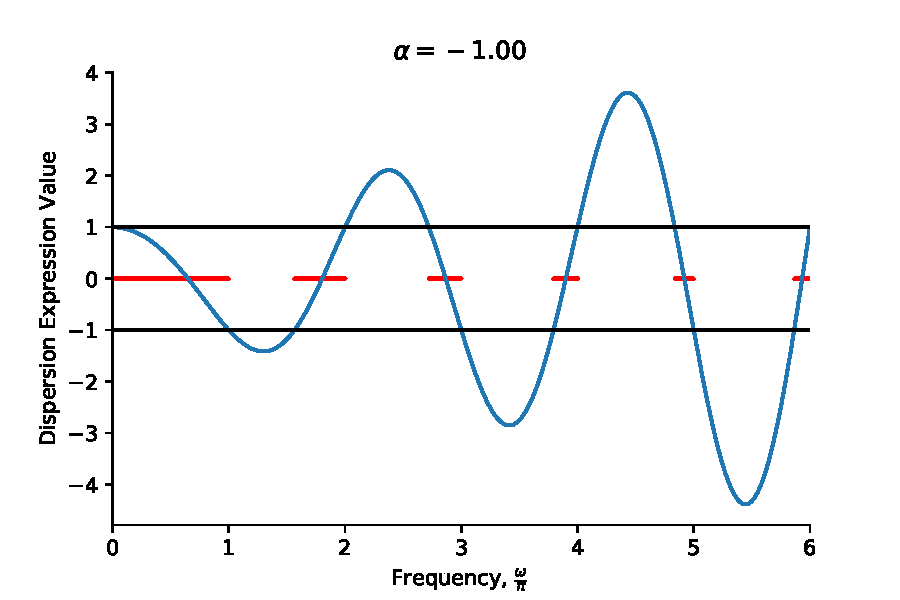
\includegraphics[scale=0.5]{Scalar_ThickVertexDR_a-1.pdf}
		\caption{\label{fig:Scalar_ThickVertexDR_a-1} The function $\Xi$ for $\alpha=-1$.}
	\end{subfigure}
	~
	\begin{subfigure}[t]{0.45\textwidth}
		\centering
		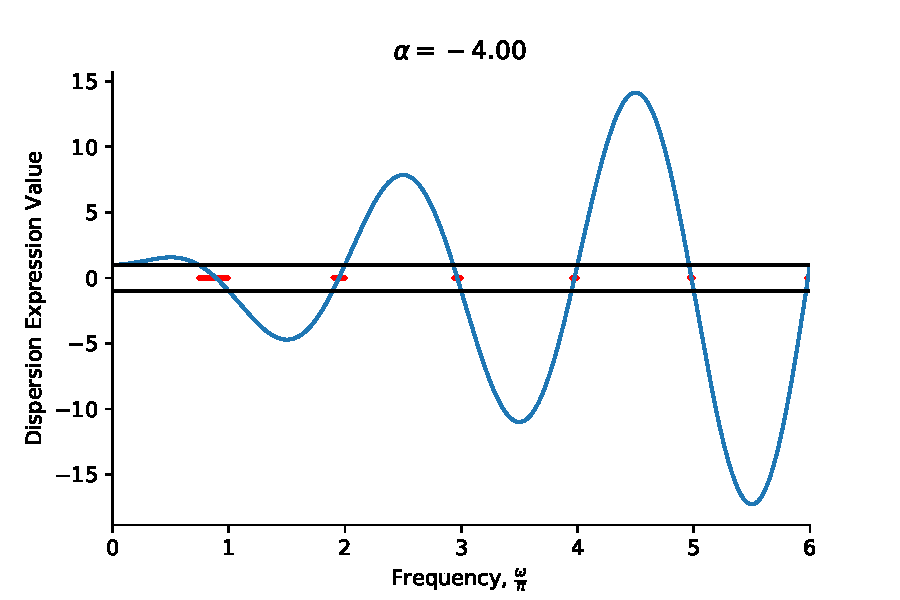
\includegraphics[scale=0.5]{Scalar_ThickVertexDR_a-4.pdf}
		\caption{\label{fig:Scalar_ThickVertexDR_a-4} The function $\Xi$ for $\alpha=-4$.}
	\end{subfigure}
	\newline
	\begin{subfigure}[t]{0.45\textwidth}
		\centering
		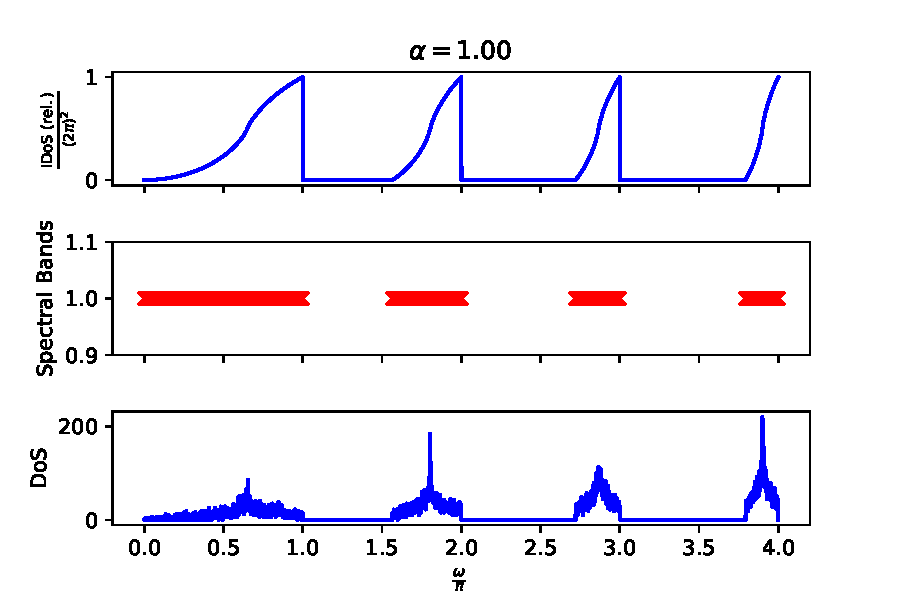
\includegraphics[scale=0.5]{CrossInPlane_DoS_Alpha1.pdf}
		\caption{\label{fig:CrossInPlane_DoS_Alpha1} The (relative) integrated density of states (IDoS), density of states (DoS) and spectrum for the system with $\alpha=1$.}
	\end{subfigure}
	~
	\begin{subfigure}[t]{0.45\textwidth}
		\centering
		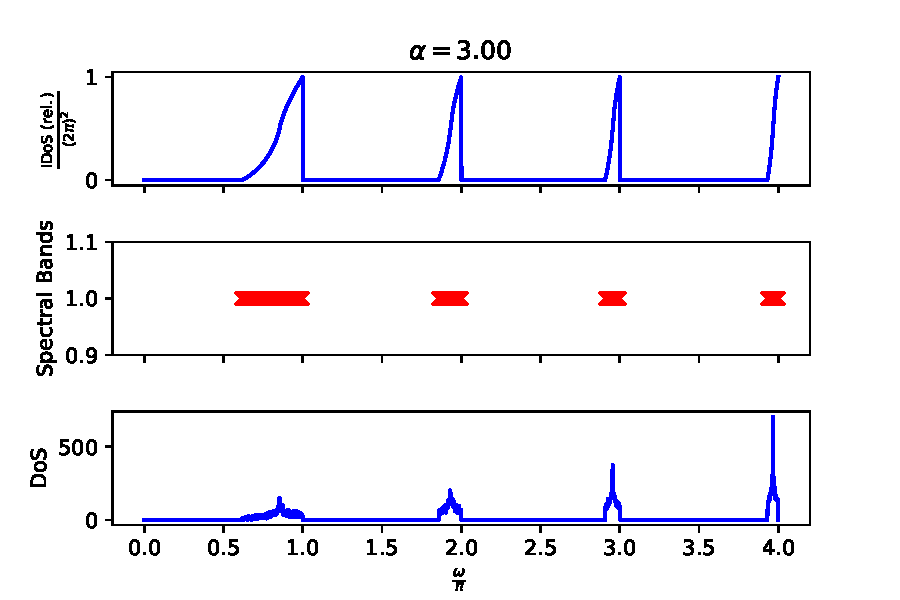
\includegraphics[scale=0.5]{CrossInPlane_DoS_Alpha3.pdf}
		\caption{\label{fig:CrossInPlane_DoS_Alpha3} The (relative) integrated density of states (IDoS), density of states (DoS) and spectrum for the system with $\alpha=3$.}
	\end{subfigure}	
	\caption{\label{fig:Scalar_ThickVertexAllResults} The function $\Xi$, and density of states for the graph topology in section \ref{ssec:ExampleCrossInPlane}.
	Red regions indicate those $\omega$ that correspond to eigenvalues $\omega^2$, when $\Xi$ takes values between $-1$ and $1$ (black lines).
	One can see the existence of spectral bands (red lines) which shrink in size as $\omega\rightarrow\infty$, with the spectrum concentrating on the centre of these bands.}
\end{figure}
We observe that the points $\omega$ that satisfy \eqref{eq:ExampleThickVertexDispExpr} are divided into distinct ``spectral bands" which shrink as $\omega\rightarrow\infty$.
The value of $\alpha$ affects whether there is a gap in the spectrum between 0 and the first spectral band; values of $\alpha<2$ result in the first band starting at 0, whilst $\alpha\geq 2$ results in a gap between zero and the bottom of the spectrum.
It can also be shown that the spectral bands are all have right-endpoints equal to a multiple of $n\pi$, although whether this endpoint is included as part of the spectrum depends on whether $n$ is even (as \eqref{eq:ExampleThickVertexSolution} only holds for $\omega\neq 2m\pi$).
We can also complement this analysis with a numerical estimate of the density of states (figures \ref{fig:CrossInPlane_DoS_Alpha1} and \ref{fig:CrossInPlane_DoS_Alpha3}) \tstk{need to define DoS?}, again confirming the existence of spectral gaps and also demonstrating that the spectrum ``concentrates" at the center of each spectral band.
\tstk{Comparison to other works on singular-structure geometries ... refs to Kirll-Sasha-Yulia's chain paper, for example, where the gap at 0 wasn't opened?}.